% Options for packages loaded elsewhere
\PassOptionsToPackage{unicode}{hyperref}
\PassOptionsToPackage{hyphens}{url}
%
\documentclass[
]{article}
\usepackage{lmodern}
\usepackage{amssymb,amsmath}
\usepackage{ifxetex,ifluatex}
\ifnum 0\ifxetex 1\fi\ifluatex 1\fi=0 % if pdftex
  \usepackage[T1]{fontenc}
  \usepackage[utf8]{inputenc}
  \usepackage{textcomp} % provide euro and other symbols
\else % if luatex or xetex
  \usepackage{unicode-math}
  \defaultfontfeatures{Scale=MatchLowercase}
  \defaultfontfeatures[\rmfamily]{Ligatures=TeX,Scale=1}
\fi
% Use upquote if available, for straight quotes in verbatim environments
\IfFileExists{upquote.sty}{\usepackage{upquote}}{}
\IfFileExists{microtype.sty}{% use microtype if available
  \usepackage[]{microtype}
  \UseMicrotypeSet[protrusion]{basicmath} % disable protrusion for tt fonts
}{}
\makeatletter
\@ifundefined{KOMAClassName}{% if non-KOMA class
  \IfFileExists{parskip.sty}{%
    \usepackage{parskip}
  }{% else
    \setlength{\parindent}{0pt}
    \setlength{\parskip}{6pt plus 2pt minus 1pt}}
}{% if KOMA class
  \KOMAoptions{parskip=half}}
\makeatother
\usepackage{xcolor}
\IfFileExists{xurl.sty}{\usepackage{xurl}}{} % add URL line breaks if available
\IfFileExists{bookmark.sty}{\usepackage{bookmark}}{\usepackage{hyperref}}
\hypersetup{
  pdftitle={Intergenerational empowerment and early sexual onset among female adolescents: Evidence from a prevalence study in Ecuador},
  pdfauthor={Alonso Quijano},
  hidelinks,
  pdfcreator={LaTeX via pandoc}}
\urlstyle{same} % disable monospaced font for URLs
\usepackage[margin=1in]{geometry}
\usepackage{graphicx}
\makeatletter
\def\maxwidth{\ifdim\Gin@nat@width>\linewidth\linewidth\else\Gin@nat@width\fi}
\def\maxheight{\ifdim\Gin@nat@height>\textheight\textheight\else\Gin@nat@height\fi}
\makeatother
% Scale images if necessary, so that they will not overflow the page
% margins by default, and it is still possible to overwrite the defaults
% using explicit options in \includegraphics[width, height, ...]{}
\setkeys{Gin}{width=\maxwidth,height=\maxheight,keepaspectratio}
% Set default figure placement to htbp
\makeatletter
\def\fps@figure{htbp}
\makeatother
\setlength{\emergencystretch}{3em} % prevent overfull lines
\providecommand{\tightlist}{%
  \setlength{\itemsep}{0pt}\setlength{\parskip}{0pt}}
\setcounter{secnumdepth}{-\maxdimen} % remove section numbering
\usepackage{dcolumn}
\usepackage{booktabs}
\usepackage{longtable}
\usepackage{array}
\usepackage{multirow}
\usepackage{wrapfig}
\usepackage{float}
\usepackage{colortbl}
\usepackage{pdflscape}
\usepackage{tabu}
\usepackage{threeparttable}
\usepackage{threeparttablex}
\usepackage[normalem]{ulem}
\usepackage{makecell}
\usepackage{xcolor}
\newlength{\cslhangindent}
\setlength{\cslhangindent}{1.5em}
\newenvironment{cslreferences}%
  {\setlength{\parindent}{0pt}%
  \everypar{\setlength{\hangindent}{\cslhangindent}}\ignorespaces}%
  {\par}

\title{Intergenerational empowerment and early sexual onset among female
adolescents: Evidence from a prevalence study in Ecuador}
\author{Alonso Quijano}
\date{}

\begin{document}
\maketitle

\emph{This study uses data from the 2018 National Health and Nutrition
Survey of Ecuador (Ensanut) to examine whether maternal sexual
empowerment is predictive of early sexual onset among female
adolescents. We used mothers' ability to turn down sex and demand
contraception as a measure of sexual empowerment. We also considered
mothers' age at first intercourse and whether they had experienced early
childbearing. Several logistic regressions were employed to estimate the
predicting value and significance of the variables of interest. Even
after controlling for several sociodemographic and economic confounders,
having a mother who lacked sexual empowerment was predictive of early
sexual activity. However, mothers' age at first intercourse was included
in the model, sexual empowerment was no longer significant, suggesting
that maternal sexual empowerment was predictive of sexual debut through
mothers' age at first intercourse. This study contributes to the
literature of early sexual initiation by exploring new connections in
which sexual values and behaviors may be transmitted from mother to
daughter. More research is needed confirm the robustness of these
results and analyze other forms of maternal empowerment.}

\hypertarget{intruduction}{%
\subsection{INTRUDUCTION}\label{intruduction}}

The age of puberty onset has decreased substantially over the past
decades (Bellis, Downing, and Ashton 2006). Reasons exist to be
concerned about this fact as early sexual debut has been linked to
several adverse outcomes. Early sexual initiators have been found to be
more prone to having multiple sex partners, forcing partners to have
sex, having frequent sexual intercourse, and being engaged in teenage
pregnancy (O'Donnell, O'Donnell, and Stueve 2001). Studies performed on
different populations have also shown an association between early
initiation of sexual intercourse and HIV and other STDs risks
(e.g.~Kaestle et al. 2005; Stöckl et al. 2013). One major cause of the
high prevalence of STDs and unwanted pregnancies among young males and
females is that those who engage in early sexual activityare much less
likely to use contraception (Finer and Philbin 2013). Additionally, even
for those who manage to avoid pregnancy at first intercourse despite not
using contraception, chances of experiencing early childbearing remain
high since those who fail to use contraception at first sex are more
likely to continue engaging in risky sexual behavior in the future (St
Lawrence and Scott 1996; Magnusson, Masho, and Lapane 2012).

Many studies have tested the relationship between precocious sexual
initiation and household structure (e.g.~Ellis et al. 2003; Newcomer and
Udry 1987) and parental involvement (e.g.~Romer et al. 1999; Sieverding
et al. 2005; Velez-Pastrana, Gonzadez-Rodriguez, and Borges-Hernandez
2005). However, few studies have explored the intergenerational
transmission of behavioral patterns, such as how the timing of sexual
debut may be replicated across generations (e.g.~Johnson and Tyler
2007). This paper aims to examine the predicting ability of maternal
behavioral variables, including the mother's age at first intercourse,
and other mechanisms in which the mother's control of her sexual
decisions can be passed on to her daughter's own decision making. It is
plausible to believe that those mothers with low bargaining power may
directly or indirectly transmit their norms and beliefs to their
daughters, who may as well then become unable to exercise
decision-making over their sexuality. Parkes et al.~(2011) found that
talking about sex and contraception with children was negatively
correlated with delayed sexual initiation, suggesting that parents may
be able to shape their children's skills for negotiating sexual
situations. The influence intra-household sexual bargaining has on
children has yet been explored in experimental research. Therefore, this
study opens up an opportunity to discuss more in depth how sexual values
may be inherited and how they can relate to the sexual well-being of
young women.

\hypertarget{methods}{%
\subsection{METHODS}\label{methods}}

\hypertarget{data-and-sample}{%
\subsection{Data and sample}\label{data-and-sample}}

We used data from the 2018 National Health and Nutrition Survey of
Ecuador (Ensanut), which is conducted every five years by the National
Statistics Institute of Ecuador. Its goal is to assess the health and
nutritional status of adults and children in Ecuador. In 2018, the
survey gathered data from 43,311 households, totaling a number of
168,747 subjects. Measures of anthropometric, nutrition, economic status
were collected for all the members of the household. Data about the
sexual health of women was gathered for all those between 12 and 49
years old. Information about risk factors (e.g.~smoking and drinking)
was collected for only one random subject (male or female) between 5 and
18.

To perform the analysis, we selected the data of girls who were 16 years
old at the time of the interview and their mothers. Because the we are
interested on how mother-related variables such as sexual empowerment
may relate to early sexual debut among young females, we filtered those
girls who were currently living with their mothers and their mothers'
partner (which in most cases was the father). As mentioned before,
information regarding sexuality was only gathered for women at age 49 or
younger. Therefore, we only considered those whose mother was under that
age threshold. Finally, as data about smoking and drinking are not
available for every subject, we decided to perform the analysis on two
samples: one larger sample that does not include these additional
confounders and a smaller one that includes them.

\hypertarget{measures}{%
\subsection{Measures}\label{measures}}

As in most studies that use secondary data, not all variables necessary
to understand the sexual activity of young females were available in
Ensanut. Nevertheless, we still were able to add several of the factors
that have been previously associated with early sexual debut.

The dependent variable for the analysis was \emph{early sexual
activity}. The 16-year-old girls who reported having had sexual
intercourse were coded as 1, whereas those who reported being virgin
were coded as 0. The 16-year-old cutoff has been used in previous
studies to demarcate early onset of sexual activity (e.g.~Ellis et al.
2003; Paul et al. 2000).

Basic sociodemographic and economic measures included ethnicity (whether
the girl identified herself as an ethnic minority), geographic area
(urban or rural), whether the girl was attending school, and household
income in US dollars. We used income as a measure of poverty. However,
evidence favors the use of consumption as a more effective tool to
measure well-being in developing countries (Meyer and Sullivan 2003).
Since consumption was not available in the survey, we added other
variables which may relate to the economic status of the household,
including access to internet and the number of household members. The
number of household members was the most predicting factor for
impoverishment used in the Poverty Probability Index (Schreiner 2015).

Individual-level measures consisted of knowledge about sexuality and
risk behaviors. Sexuality knowledge was estimated through questions
about menstruation, pregnancy, and AIDs. Girls were asked whether they
knew what was happening to their body when they hay their first period,
whether a woman could become pregnant at first intercourse, and whether
HIV could spread through handshake. They were also asked whether they
had ever learned about sexual relations, and if so, from whom they had
learned about (school, family, and others). Risk factors included
whether the girl had ever drunk alcohol or smoked in the past.

Mother-related variables included the mother's sexual bargaining
ability, age at first intercourse, and whether she had a teenage birth.
Mothers were asked if they could say no to their sexual partners
whenever they did not want to have sexual intercourse. For those who
were not using any form of contraception but would prefer to use one,
they were asked whether they thought their partner would be willing to
use it or not. Mothers who were unable to turn down sex or demand their
partner to use contraception were classified as low sexual bargaining.
We also considered variables such as occupation and education.

\hypertarget{results}{%
\subsection{RESULTS}\label{results}}

After cleaning up the data, the sample contained answers from 828
16-year-old girls and their respective mothers. Among those, 16.4\% had
ever had sexual intercourse, while 83.6\% had not. Before performing the
primary analysis, differences in the prevalence of early sexual onset
and their relationship with the explanatory variables were assessed
using the chi-square and t-test. The primary analysis was based on a
series of logistic regression models examining the association between
early sexual activity among young females and the characteristics of
their mothers after adjustment for covariates.

Table 1 shows the percentage and mean levels of the explanatory
variables by each group. Mean differences of the categorical and
continuous variables were tested using the chi-square and t-test,
respectively. Across the two groups, girls who were sexually active were
more likely to belong to an ethnic minority (p \textless{} .001), live
in a rural area (p \textless{} .05), lack internet access (p \textless{}
.001), and miss school (p \textless{} .001). As for sexuality knowledge,
they tended to incorrectly answer the question about AIDs (p \textless{}
.05) and not know what was happening to their body when they had their
first period (p \textless{} .001). Sexually active girls were more
likely to learn about sexuality from family (p \textless{} .05) and
other sources (e.g., internet) (p \textless{} .001). In contrast,
non-sexually active girls were more prone to learning from school (p
\textless{} .001).

\begin{table}

\caption{\label{tab:unnamed-chunk-1}Percentage and mean levels of explanatory variables by group}
\centering
\begin{threeparttable}
\begin{tabular}[t]{lrrl}
\toprule
Variables & Early sexual activity & No early sexual activity & p value\\
\midrule
Ethnic minority & 0.30 & 0.21 & 0.001 ***\\
Lives in a rural area & 0.48 & 0.41 & 0.033 **\\
Does not have internet & 0.75 & 0.55 & 0.000 ***\\
Misses school & 0.44 & 0.05 & 0.000 ***\\
Lacks knowledge about period & 0.28 & 0.19 & 0.000 ***\\
\addlinespace
Lacks knowledge about pregnancy & 0.20 & 0.17 & 0.273\\
Lacks knowledge about AIDs & 0.18 & 0.12 & 0.014 **\\
Does not know about sexuality & 0.09 & 0.07 & 0.273\\
Knows about sexuality from family & 0.15 & 0.10 & 0.015 **\\
Knows about sexuality from school & 0.68 & 0.80 & 0.000 ***\\
\addlinespace
Knows about sexuality from other sources & 0.08 & 0.03 & 0.000 ***\\
Has ever drunk alcohol & 0.62 & 0.44 & 0.000 ***\\
Has ever smoked & 0.09 & 0.03 & 0.000 ***\\
Mother has a job & 0.64 & 0.60 & 0.282\\
Mother finished primary school & 0.91 & 0.96 & 0.003 ***\\
\addlinespace
Mother finished high school & 0.44 & 0.51 & 0.1  *\\
Mother finished college & 0.09 & 0.16 & 0.021 **\\
Mother had a teenage birth & 0.68 & 0.48 & 0.000 ***\\
Mother lacks sexual bargaining & 0.15 & 0.11 & 0.108\\
Household income & 646.79 & 630.03 & 0.944\\
\addlinespace
Number of members in the household & 5.64 & 5.42 & 0.08  *\\
Mother's age at first intercourse & 16.11 & 17.64 & 0.000 ***\\
\bottomrule
\end{tabular}
\begin{tablenotes}[para]
\item \textit{Note: } 
\item p values for comparison of percentagges using chi-square. p values for comparison of means using t-test. Ns = 401–828. *p < .1; **p < .05; ***p < .01
\end{tablenotes}
\end{threeparttable}
\end{table}

Mother characteristics significantly differed across groups. Mothers of
early sexual initiators were less likely to have finished primary school
(p \textless{} .01) and more likely to have become a teenage parent (p
\textless{} .001). As expected, early sexual initiators were more likely
to have been reared by a mother who had herself had her first coitus at
a very young age. Figure 1 illustrates the cumulative histogram of age
at first coitus of the mothers. The figure clearly shows that mothers of
early sexual initiators had their first coitus at a younger age than
mothers of those who were not sexually active. The mean age at first
coitus for each group was 16.11 (SD = 2.48) and 17.76 (SD = 2.79),
respectively. The t-test showed that these differences were unlikely to
have been due to chance (p \textless{} .001).

\begin{figure}

{\centering 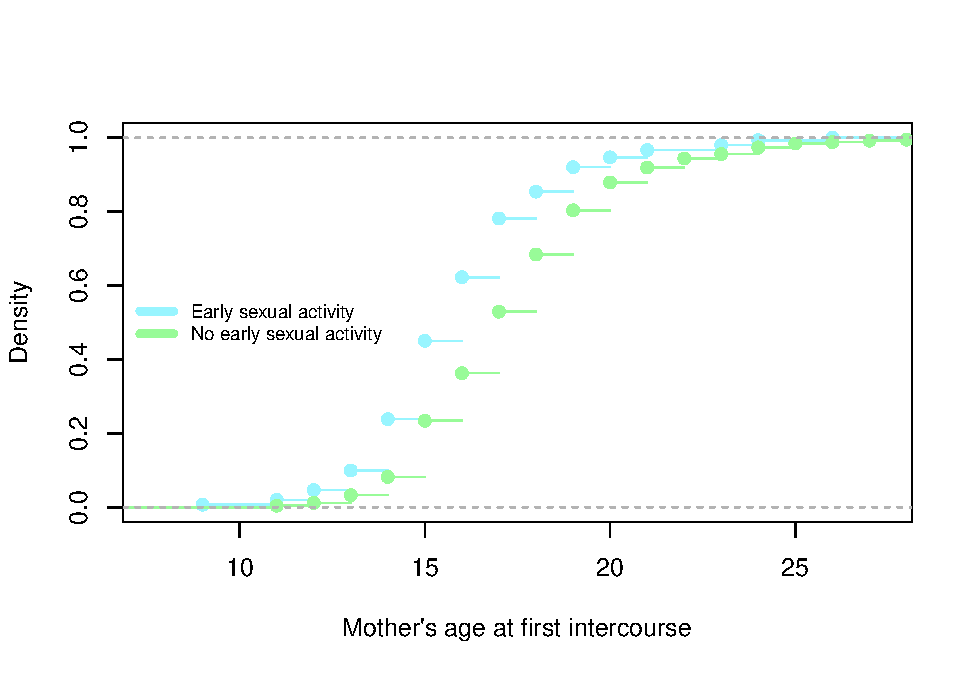
\includegraphics[width=0.8\linewidth,height=0.7\textheight]{early_sexual_activity_report_files/figure-latex/unnamed-chunk-2-1} 

}

\caption{Cumulative histogram of age at first intercourse of mothers by group}\label{fig:unnamed-chunk-2}
\end{figure}

Logistic regressions were used to assess the relationship between the
early onset of sexual activity among girls and the mothers' sexual
bargaining ability, as well as other behavioral traits such as the
mothers' age at first intercourse and whether she had a teenage birth.
Table 2 shows the coefficients (log odds ratio) of these regressions. To
observe the predicting ability of the three mother-related variables
(sexual bargaining, teenage birth, and age at first intercourse) alone
and in interaction, we computed three logistic regressions. Thus, we can
notice how the significance of the coefficient changes with each
additional variable. Each regression is represented by a separate column
in Table 2.

As demonstrated in column 2 of Table 2, after adjustment for all
covariates, having a mother who lacks sexual bargaining and a mother who
had a teenage birth significantly increases the log odds of early sexual
onset. These results support the hypothesis that the sexual attitudes
and behavior may be in some mechanism inherited from mother to daughter.
Similarly, column 3 of Table 2 shows that for each additional year that
the mother delays her sexual debut, the log odds of her daughter being
sexually active decrease. When the age at first intercourse of the
mother is added to the model, however, lacking sexual bargaining and
having a teenage birth become statistically insignificant due to the
correlation of predictors. A plausible explanation is that the age at
first intercourse explains whether the mother is sexually empowered and
whether she was once a teenage mother.

Although not the main focus of the study, it is worth examining whether
sexuality knowledge has a predictive value in the model. As shown in
Table 2, while knowledge about period, pregnancy, and AIDs are not
statistically significant in any of the regressions, from whom girls
acquire information about sexual relations seems to matter. Even after
controlling for school attendance and other covariates, girls who learn
about sex from family have higher odds of engaging in early sexual
activity than those who learn from school. It is also worth noting that
the sociodemographic variables do not appear to explain the differences
in early sexual onset. In contrast, missing school and having an
employed mother significantly increases the logs odds of early sexual
debut.

As mentioned before, data about smoking and drinking were not gathered
for all subjects in our sample. Therefore, a series of logistic
regressions were performed on a smaller sample in order to add the two
cofounders to the original model. These regressions are illustrated in
Table 3. However, it is important to emphasize that the probability of
falling into type 2 error increases as the sample becomes smaller. Thus,
while having more cofounders improves the accuracy of the outcomes,
reducing the sample size may as well affect the precision of the
estimates.

As expected, smoking and drinking were high predictors for precocious
sexual initiation. Table 3 shows that even after controlling for these
two additional variables, the log odds of early sexual onset decrease
for each additional year that the mother delays her sexual debut.
Interestingly, when adding these cofounders, from whom girls learn about
sexual relations and having an employed mother are no longer
significant. As with the previous regressions, attending school and
having a mother who finished primary school are associated with delayed
sexual activity.

\begin{table}[!htbp] \centering 
  \caption{Logistic Regression Results} 
  \label{} 
\begin{tabular}{@{\extracolsep{5pt}}lD{.}{.}{-3} D{.}{.}{-3} D{.}{.}{-3} } 
\\[-1.8ex]\hline 
\hline \\[-1.8ex] 
 & \multicolumn{3}{c}{\textit{Dependent variable:}} \\ 
\cline{2-4} 
\\[-1.8ex] & \multicolumn{3}{c}{Early sexual activity} \\ 
\\[-1.8ex] & \multicolumn{1}{c}{(1)} & \multicolumn{1}{c}{(2)} & \multicolumn{1}{c}{(3)}\\ 
\hline \\[-1.8ex] 
 Ethnic minority & 0.314 & 0.324 & 0.325 \\ 
  & (0.255) & (0.259) & (0.270) \\ 
  Lives in a rural area & -0.053 & -0.025 & 0.058 \\ 
  & (0.231) & (0.233) & (0.241) \\ 
  Household income & 0.0001 & 0.0001 & 0.0001 \\ 
  & (0.0001) & (0.0001) & (0.0001) \\ 
  Number of members in the household & 0.098 & 0.070 & 0.037 \\ 
  & (0.056) & (0.058) & (0.059) \\ 
  Does not have internet & 0.430 & 0.447 & 0.404 \\ 
  & (0.246) & (0.249) & (0.257) \\ 
  Misses school & 2.127^{***} & 2.139^{***} & 2.163^{***} \\ 
  & (0.319) & (0.322) & (0.340) \\ 
  Lacks knowledge about period & 0.251 & 0.242 & 0.350 \\ 
  & (0.252) & (0.254) & (0.264) \\ 
  Lacks knowledge about pregnancy & 0.290 & 0.323 & 0.424 \\ 
  & (0.260) & (0.261) & (0.272) \\ 
  Lacks knowledge about AIDs & -0.024 & 0.033 & -0.120 \\ 
  & (0.308) & (0.311) & (0.337) \\ 
  Knows about sexuality from family & 2.631^{*} & 2.578^{*} & 2.564^{*} \\ 
  & (1.141) & (1.205) & (1.204) \\ 
  Knows about sexuality from school & 2.069 & 2.125 & 2.056 \\ 
  & (1.109) & (1.173) & (1.170) \\ 
  Knows about sexuality from other sources & 3.000^{*} & 2.976^{*} & 3.144^{*} \\ 
  & (1.191) & (1.250) & (1.248) \\ 
  Mother has a job & 0.631^{**} & 0.575^{*} & 0.595^{*} \\ 
  & (0.225) & (0.228) & (0.236) \\ 
  Mother finished primary school & -1.187 & -1.332 & -1.161 \\ 
  & (0.683) & (0.695) & (0.707) \\ 
  Mother finished secondary school & -0.693 & -0.790 & -0.584 \\ 
  & (0.685) & (0.697) & (0.710) \\ 
  Mother finished college & -0.943 & -0.961 & -0.554 \\ 
  & (0.734) & (0.744) & (0.761) \\ 
  Mother lacks sexual bargaining & 0.628^{*} & 0.600^{*} & 0.478 \\ 
  & (0.297) & (0.300) & (0.316) \\ 
  Mother had a teenage birth &  & 0.778^{***} & 0.294 \\ 
  &  & (0.220) & (0.258) \\ 
  Mother's age at first intercourse &  &  & -0.188^{***} \\ 
  &  &  & (0.055) \\ 
  Constant & -4.583^{***} & -4.829^{***} & -1.389 \\ 
  & (1.287) & (1.334) & (1.649) \\ 
 \hline \\[-1.8ex] 
Observations & \multicolumn{1}{c}{828} & \multicolumn{1}{c}{824} & \multicolumn{1}{c}{783} \\ 
Log Likelihood & \multicolumn{1}{c}{-321.446} & \multicolumn{1}{c}{-314.520} & \multicolumn{1}{c}{-291.948} \\ 
Akaike Inf. Crit. & \multicolumn{1}{c}{678.891} & \multicolumn{1}{c}{667.040} & \multicolumn{1}{c}{623.895} \\ 
\hline 
\hline \\[-1.8ex] 
\textit{Note:}  & \multicolumn{3}{r}{$^{*}$p$<$0.05; $^{**}$p$<$0.01; $^{***}$p$<$0.001} \\ 
\end{tabular} 
\end{table}

\begin{table}[!htbp] \centering 
  \caption{Logistic Regression Results} 
  \label{} 
\begin{tabular}{@{\extracolsep{5pt}}lD{.}{.}{-3} D{.}{.}{-3} D{.}{.}{-3} } 
\\[-1.8ex]\hline 
\hline \\[-1.8ex] 
 & \multicolumn{3}{c}{\textit{Dependent variable:}} \\ 
\cline{2-4} 
\\[-1.8ex] & \multicolumn{3}{c}{Early sexual activity} \\ 
\\[-1.8ex] & \multicolumn{1}{c}{(1)} & \multicolumn{1}{c}{(2)} & \multicolumn{1}{c}{(3)}\\ 
\hline \\[-1.8ex] 
 Ethnic minority & 0.671 & 0.695 & 0.667 \\ 
  & (0.409) & (0.411) & (0.414) \\ 
  Lives in a rural area & -0.411 & -0.372 & -0.363 \\ 
  & (0.354) & (0.354) & (0.358) \\ 
  Household income & 0.0002 & 0.0002 & 0.0002 \\ 
  & (0.0001) & (0.0001) & (0.0001) \\ 
  Number of members in the household & 0.118 & 0.095 & 0.087 \\ 
  & (0.091) & (0.093) & (0.093) \\ 
  Does not have internet & 0.775^{*} & 0.774^{*} & 0.675 \\ 
  & (0.357) & (0.356) & (0.358) \\ 
  Misses school & 1.554^{**} & 1.532^{**} & 1.568^{**} \\ 
  & (0.495) & (0.498) & (0.513) \\ 
  Lacks knowledge about period & -0.232 & -0.199 & -0.168 \\ 
  & (0.426) & (0.427) & (0.434) \\ 
  Lacks knowledge about pregnancy & -0.165 & -0.174 & -0.122 \\ 
  & (0.434) & (0.435) & (0.437) \\ 
  Lacks knowledge about AIDs & -0.007 & -0.037 & -0.208 \\ 
  & (0.505) & (0.510) & (0.524) \\ 
  Knows about sexuality from family & 1.288 & 1.329 & 1.244 \\ 
  & (1.585) & (1.623) & (1.623) \\ 
  Knows about sexuality from school & 0.659 & 0.771 & 0.636 \\ 
  & (1.537) & (1.578) & (1.580) \\ 
  Knows about sexuality from other sources & 1.656 & 1.755 & 1.623 \\ 
  & (1.648) & (1.684) & (1.683) \\ 
  Mother has a job & 0.488 & 0.436 & 0.455 \\ 
  & (0.325) & (0.327) & (0.333) \\ 
  Mother finished primary school & -2.610^{**} & -2.748^{**} & -2.460^{*} \\ 
  & (0.971) & (0.979) & (0.981) \\ 
  Mother finished secondary school & -2.018^{*} & -2.128^{*} & -1.782 \\ 
  & (0.980) & (0.984) & (0.987) \\ 
  Mother finished college & -2.215^{*} & -2.275^{*} & -1.792 \\ 
  & (1.047) & (1.046) & (1.057) \\ 
  Ever drunk alcohol & 0.872^{**} & 0.868^{**} & 0.785^{*} \\ 
  & (0.328) & (0.328) & (0.333) \\ 
  Ever smoked & 1.415^{**} & 1.358^{**} & 1.404^{**} \\ 
  & (0.497) & (0.500) & (0.512) \\ 
  Mother lacks sexual bargaining & 0.685 & 0.704 & 0.587 \\ 
  & (0.438) & (0.440) & (0.450) \\ 
  Mother had a teenage birth &  & 0.353 & -0.131 \\ 
  &  & (0.311) & (0.358) \\ 
  Mother's age at first intercourse &  &  & -0.191^{*} \\ 
  &  &  & (0.080) \\ 
  Constant & -2.446 & -2.483 & 0.998 \\ 
  & (1.749) & (1.782) & (2.272) \\ 
 \hline \\[-1.8ex] 
Observations & \multicolumn{1}{c}{417} & \multicolumn{1}{c}{415} & \multicolumn{1}{c}{401} \\ 
Log Likelihood & \multicolumn{1}{c}{-155.455} & \multicolumn{1}{c}{-154.608} & \multicolumn{1}{c}{-150.149} \\ 
Akaike Inf. Crit. & \multicolumn{1}{c}{350.910} & \multicolumn{1}{c}{351.216} & \multicolumn{1}{c}{344.298} \\ 
\hline 
\hline \\[-1.8ex] 
\textit{Note:}  & \multicolumn{3}{r}{$^{*}$p$<$0.05; $^{**}$p$<$0.01; $^{***}$p$<$0.001} \\ 
\end{tabular} 
\end{table}

\hypertarget{discussion}{%
\subsection{DISCUSSION}\label{discussion}}

This study contributes to the literature on early initiation of sexual
activity among female adolescents. It is not the time maternal
empowerment has been studied as a predictor of sexual activity. Gipson
and Upchurch (2017), for instance, found that some of characteristics
and measures of maternal empowerment and status were predictive of their
daughters' sexual initiation. Yet, few if any have explored maternal
empowerment in the way it has been done in this study. In this research,
we found that girls who had a mother that was unable to turn down sex or
demand the use of contraception were more likely to be sexually active.
This raises the question of whether women's sexual behavior or
empowerment can be transmitted intergenerationally. It is worth noting
that sexual coercion is still a major cause of sexual debut (Moore et
al. 2007). In our sample, 34\% of girls reported not having agreed or
being convinced to engage in sexual activity at the time of their first
sexual experience. Perhaps, young women are able to mimic the sexual
conduct of their mothers. If submissive behavior is normalized within
the family, girls may find it acceptable to receive and accept sexual
advances against their will.

Another important outcome of this research was the relationship between
the timing of sexual onset among mothers and daughters. Even after
controlling for several cofounders, the mother's age at sexual debut was
one of the most significant and independent predictors. The younger a
mother was when she had her first intercourse, the higher the odds of
her daughter being sexually active by the age of 16. This finding is
parallel to the intergenerational tendency of early childbearing (Kahn
and Anderson 1992), in which teenage mothers are more likely to have
been brought up by a single mother who had herself become a parent early
in her life. Previous research on sexual initiation has found that
adding drug use as a covariate largely impacts the significance of
coefficients (e.g.~Mandara, Murray, and Bangi 2003). However, when
smoking and drinking were added into our models, the mother's age at
first intercourse remained statistically significant.

It is also worth discussing the interaction between sexual bargaining
and sexual onset among mothers. The mothers' sexual bargaining was a
good predictor of their daughters' sexual activity in the first models.
Nevertheless, when combined with the mothers' age at first coitus,
sexual bargaining was no longer significant, implying that sexual
bargaining predicted sexual activity through age at first coitus. These
findings strengthen the hypothesis of maternal empowerment as a
potential determinant of the timing of sexual debut. How much control
mothers have of their own sexual decision making may be mirrored in
their daughters' behavior. Mothers who started their sexual life
prematurely may have done so for reasons not necessarily attached to
their choice. These assumptions, however, need to be corroborated with
future research.

We found that girls whose mothers had completed primary school were less
likely to have engaged in sexual intercourse. These results are
consistent with previous evidence that has shown that maternal education
inhibits the risk of early sexual debut (e.g.~Brewster 1994; Jordahl and
Lohman 2009; Santelli et al. 2000). One explanation that has been
proposed is that better-educated parents have higher expectations for
their children to finish school and establish a career, putting pressure
on them to delay sexual onset (Guo et al. 2012). We also found that the
source from which girls received information about sexuality was a good
predictor of their sexual behavior. After controlling for school
attendance, girls who learned about sexuality from family were more
likely to have experienced sexual activity than their peers who reported
having learned from school. In Ecuador, parents have shown interest in
addressing sexuality with their children in order to discourage them
from having sexual relations. Yet, they face a few constraints,
including lack of knowledge and feelings of shame and anxiety (Jerves et
al. 2014). These limitations may hinder these efforts and even produce
unintended results. This may be one of the explanations why
communication from parent to child about sex was predictive of early
sexual activity.

To control for socioeconomic status, we also included measures such as
household income, access to internet, and household members. For
better-off households, we suspected that having a higher economic level
would likely increase the opportunity of having sexual relations
(e.g.~pregnancy). Yet, none of these variables was strongly predictive
of sexual debut. As for the mothers' employment, while we thought that
having a job would reduce the odds of precocious sexual initiation, we
found the opposite. Since the purpose of the survey was to gather data
about health and nutrition, it did not collect information about
parental monitoring. However, employed mothers may spend less time
supervising or parenting their daughters. Research findings are most
consistent that mother-child closeness and values towards sexual
relations are associated with lower risk of sexual activity (Sieving,
McNeely, and Blum 2000).

Studies have shown that smoking and substance use among adolescents are
associated with early sexual activity (Bachanas et al. 2002; Mandara,
Murray, and Bangi 2003; Robinson, Teiljohann, and Price 1999). In this
study, we conducted a series of separate models in which we included
smoking and drinking as cofounders. We had to reduce the sample size as
data about these specific risk factors were only obtained for a smaller
group of subjects. Yet, after adding these variables, the computed
estimates were large and significant. These findings corroborate
previous research showing that substance use plays a critical role in
adolescents' sexual decisions. Bachanas et al.~(2002) explored the
predictive ability of peer norms and substance use. They found that
while both variables were significantly associated with risky sexual
behavior, only substance use accounted for the variance in sexual
behavior when combined in the same model. Similarly, when we added
smoking and drinking to the regressions, communication about sexuality
became no longer significant. These results suggest that communication
about sexuality was predictive of sexual activity through substance use.
Perhaps, parents who identify deviant behavior in their children also
include conversation about sex when dealing with misconduct.

\hypertarget{conclusion}{%
\subsection{CONCLUSION}\label{conclusion}}

In this article, we discussed how maternal sexual empowerment was
related to female adolescents' sexual behavior. After controlling for
several confounders, we found that having a mother unable to turn down
sex or demand contraception increased the odds of early sexual
initiation. We also found that when adding mothers' age at first
intercourse, sexual empowerment was no longer significant. This suggests
that maternal sexual empowerment was predictive of sexual onset through
mothers' age at first intercourse. Perhaps, mothers who reported low
sexual empowerment did not have control of their sexual decisions at the
time of their first sexual encounter. We believe that in some manner,
these attitudes and values can be transmitted from mother to daughter.

Although the nature of this research does not allow for a causal
relationship to be established, we believe that female adolescents'
attitudes toward sex and the ability to refuse sexual intercourse may be
shaped somehow through their mothers' bargaining power in sexual
relationships. The traditional parental interventions designed to delay
sexual onset and promote contraception use focuses on improving
communication about sexuality. Yet, the results presented indicate that
interventions towards mothers' sexual empowerment may help girls,
especially at a very young age, to develop skills for managing sexual
relationships. New mechanisms in which maternal empowerment influences
daughters' outcomes yet need to be researched.

\hypertarget{references}{%
\subsection*{References}\label{references}}
\addcontentsline{toc}{subsection}{References}

\hypertarget{refs}{}
\begin{cslreferences}
\leavevmode\hypertarget{ref-bachanas2002predictors}{}%
Bachanas, Pamela J, Mary K Morris, Jennifer K Lewis-Gess, Eileen J
Sarett-Cuasay, Kimberly Sirl, Julie K Ries, and Mary K Sawyer. 2002.
``Predictors of Risky Sexual Behavior in African American Adolescent
Girls: Implications for Prevention Interventions.'' \emph{Journal of
Pediatric Psychology} 27 (6): 519--30.

\leavevmode\hypertarget{ref-bellis2006adults}{}%
Bellis, Mark A, J Downing, and JR Ashton. 2006. ``Adults at 12? Trends
in Puberty and Their Public Health Consequences.'' BMJ Publishing Group
Ltd.

\leavevmode\hypertarget{ref-brewster1994race}{}%
Brewster, Karin L. 1994. ``Race Differences in Sexual Activity Among
Adolescent Women: The Role of Neighborhood Characteristics.''
\emph{American Sociological Review}, 408--24.

\leavevmode\hypertarget{ref-ellis2003does}{}%
Ellis, Bruce J, John E Bates, Kenneth A Dodge, David M Fergusson, L John
Horwood, Gregory S Pettit, and Lianne Woodward. 2003. ``Does Father
Absence Place Daughters at Special Risk for Early Sexual Activity and
Teenage Pregnancy?'' \emph{Child Development} 74 (3): 801--21.

\leavevmode\hypertarget{ref-finer2013sexual}{}%
Finer, Lawrence B, and Jesse M Philbin. 2013. ``Sexual Initiation,
Contraceptive Use, and Pregnancy Among Young Adolescents.''
\emph{Pediatrics} 131 (5): 886--91.

\leavevmode\hypertarget{ref-gipson2017status}{}%
Gipson, Jessica D, and Dawn M Upchurch. 2017. ``Do the Status and
Empowerment of Mothers Predict Their Daughters' Reproductive Outcomes?''
\emph{BMC Pregnancy and Childbirth} 17 (2): 348.

\leavevmode\hypertarget{ref-guo2012timing}{}%
Guo, Wei, Zheng Wu, Yue Qiu, Gong Chen, and Xiaoying Zheng. 2012. ``The
Timing of Sexual Debut Among Chinese Youth.'' \emph{International
Perspectives on Sexual and Reproductive Health}, 196--204.

\leavevmode\hypertarget{ref-jerves2014understanding}{}%
Jerves, Elena, Silvia Lopez, Cecilia Castro, William Ortiz, Maria
Palacios, Peter Rober, and Paul Enzlin. 2014. ``Understanding Parental
Views of Adolescent Sexuality and Sex Education in Ecuador: A
Qualitative Study.'' \emph{Sex Education} 14 (1): 14--27.

\leavevmode\hypertarget{ref-johnson2007adolescent}{}%
Johnson, Katherine A, and Kimberly A Tyler. 2007. ``Adolescent Sexual
Onset: An Intergenerational Analysis.'' \emph{Journal of Youth and
Adolescence} 36 (7): 939--49.

\leavevmode\hypertarget{ref-jordahl2009bioecological}{}%
Jordahl, Tina, and Brenda J Lohman. 2009. ``A Bioecological Analysis of
Risk and Protective Factors Associated with Early Sexual Intercourse of
Young Adolescents.'' \emph{Children and Youth Services Review} 31 (12):
1272--82.

\leavevmode\hypertarget{ref-kaestle2005young}{}%
Kaestle, Christine E, Carolyn T Halpern, William C Miller, and Carol A
Ford. 2005. ``Young Age at First Sexual Intercourse and Sexually
Transmitted Infections in Adolescents and Young Adults.'' \emph{American
Journal of Epidemiology} 161 (8): 774--80.

\leavevmode\hypertarget{ref-kahn1992intergenerational}{}%
Kahn, Joan R, and Kay E Anderson. 1992. ``Intergenerational Patterns of
Teenage Fertility.'' \emph{Demography} 29 (1): 39--57.

\leavevmode\hypertarget{ref-magnusson2012early}{}%
Magnusson, Brianna M, Saba W Masho, and Kate L Lapane. 2012. ``Early Age
at First Intercourse and Subsequent Gaps in Contraceptive Use.''
\emph{Journal of Women's Health} 21 (1): 73--79.

\leavevmode\hypertarget{ref-mandara2003predictors}{}%
Mandara, Jelani, Carolyn B Murray, and Audrey K Bangi. 2003.
``Predictors of African American Adolescent Sexual Activity: An
Ecological Framework.'' \emph{Journal of Black Psychology} 29 (3):
337--56.

\leavevmode\hypertarget{ref-meyer2003measuring}{}%
Meyer, Bruce D, and James X Sullivan. 2003. ``Measuring the Well-Being
of the Poor Using Income and Consumption.'' National Bureau of Economic
Research.

\leavevmode\hypertarget{ref-moore2007coerced}{}%
Moore, Ann M, Kofi Awusabo-Asare, Nyovani Madise, Johannes John-Langba,
and Akwasi Kumi-Kyereme. 2007. ``Coerced First Sex Among Adolescent
Girls in Sub-Saharan Africa: Prevalence and Context.'' \emph{African
Journal of Reproductive Health} 11 (3): 62.

\leavevmode\hypertarget{ref-newcomer1987parental}{}%
Newcomer, Susan, and J Richard Udry. 1987. ``Parental Marital Status
Effects on Adolescent Sexual Behavior.'' \emph{Journal of Marriage and
the Family}, 235--40.

\leavevmode\hypertarget{ref-o2001early}{}%
O'Donnell, Lydia, Carl R O'Donnell, and Ann Stueve. 2001. ``Early Sexual
Initiation and Subsequent Sex-Related Risks Among Urban Minority Youth:
The Reach for Health Study.'' \emph{Family Planning Perspectives},
268--75.

\leavevmode\hypertarget{ref-parkes2011parenting}{}%
Parkes, Alison, Marion Henderson, Daniel Wight, and Catherine Nixon.
2011. ``Is Parenting Associated with Teenagers' Early Sexual
Risk-Taking, Autonomy and Relationship with Sexual Partners?''
\emph{Perspectives on Sexual and Reproductive Health} 43 (1): 30--40.

\leavevmode\hypertarget{ref-paul2000determinants}{}%
Paul, Charlotte, Julie Fitzjohn, Peter Herbison, and Nigel Dickson.
2000. ``The Determinants of Sexual Intercourse Before Age 16.''
\emph{Journal of Adolescent Health} 27 (2): 136--47.

\leavevmode\hypertarget{ref-robinson1999predictors}{}%
Robinson, K Lynne, Susan K Teiljohann, and James H Price. 1999.
``Predictors of Sixth Graders Engaging in Sexual Intercourse.''
\emph{Journal of School Health} 69 (9): 369--75.

\leavevmode\hypertarget{ref-romer1999parental}{}%
Romer, Daniel, Bonita Stanton, Jennifer Galbraith, Susan Feigelman,
Maureen M Black, and Xiaoming Li. 1999. ``Parental Influence on
Adolescent Sexual Behavior in High-Poverty Settings.'' \emph{Archives of
Pediatrics \& Adolescent Medicine} 153 (10): 1055--62.

\leavevmode\hypertarget{ref-santelli2000association}{}%
Santelli, John S, Richard Lowry, Nancy D Brener, and Leah Robin. 2000.
``The Association of Sexual Behaviors with Socioeconomic Status, Family
Structure, and Race/Ethnicity Among Us Adolescents.'' \emph{American
Journal of Public Health} 90 (10): 1582.

\leavevmode\hypertarget{ref-schreiner2015ecuador}{}%
Schreiner, Mark. 2015. ``Ecuador 2013 Poverty Probability Index(PPI):
Design Memo.''

\leavevmode\hypertarget{ref-sieverding2005influence}{}%
Sieverding, John A, Nancy Adler, Stephanie Witt, and Jonathan Ellen.
2005. ``The Influence of Parental Monitoring on Adolescent Sexual
Initiation.'' \emph{Archives of Pediatrics \& Adolescent Medicine} 159
(8): 724--29.

\leavevmode\hypertarget{ref-sieving2000maternal}{}%
Sieving, Renee E, Clea S McNeely, and Robert Wm Blum. 2000. ``Maternal
Expectations, Mother-Child Connectedness, and Adolescent Sexual Debut.''
\emph{Archives of Pediatrics \& Adolescent Medicine} 154 (8): 809--16.

\leavevmode\hypertarget{ref-st1996examination}{}%
St Lawrence, Janet S, and Catina P Scott. 1996. ``Examination of the
Relationship Between African American Adolescents' Condom Use at Sexual
Onset and Later Sexual Behavior: Implications for Condom Distribution
Programs.'' \emph{AIDS Education and Prevention}.

\leavevmode\hypertarget{ref-stockl2013early}{}%
Stöckl, Heidi, Naira Kalra, Jantine Jacobi, and Charlotte Watts. 2013.
``Is Early Sexual Debut a Risk Factor for Hiv Infection Among Women in
Sub-Saharan Africa? A Systematic Review.'' \emph{American Journal of
Reproductive Immunology} 69: 27--40.

\leavevmode\hypertarget{ref-velez2005family}{}%
Velez-Pastrana, Maria C, Rafael A Gonzadez-Rodriguez, and Adalisse
Borges-Hernandez. 2005. ``Family Functioning and Early Onset of Sexual
Intercourse in Latino Adolescents.'' \emph{Adolescence} 40 (160).
\end{cslreferences}

\end{document}
